
\chapter{Analog electronic instrumentation}

An ``analog'' electronic signal is a voltage or current proportionate to the value of some physical measurement or control quantity.  An instrument is often classified as being ``analog'' simply by virtue of using an analog signal standard to communicate information, even if the internal construction and design of the instrument may be mostly digital in nature.  This is to distinguish such instruments from those making use of no analog electronic signals at all (e.g. wireless or Fieldbus instruments).

\section{4 to 20 mA analog current signals}

The most popular form of signal transmission used in modern industrial instrumentation systems (as of this writing) is the 4 to 20 milliamp DC standard.  This is an \textit{analog} signal standard, meaning that the electric current is used to proportionately represent measurements or command signals.  Typically, a 4 milliamp current value represents 0\% of scale, a 20 milliamp current value represents 100\% of scale, and any current value in between 4 and 20 milliamps represents a commensurate percentage in between 0\% and 100\%.  The following table shows the corresponding current and percentage values for each 25\% increment between 0\% and 100\%.  Every instrument technician tasked with maintaining 4-20 mA instruments commits these values to memory, because they are referenced so often: \index{4 to 20 mA}

% No blank lines allowed between lines of an \halign structure!
% I use comments (%) instead, so that TeX doesn't choke.

$$\vbox{\offinterlineskip
\halign{\strut
\vrule \quad\hfil # \ \hfil & 
\vrule \quad\hfil # \ \hfil \vrule \cr
\noalign{\hrule}
%
% First row
\textbf{Current value} & \textbf{\% of scale} \cr
%
\noalign{\hrule}
%
% Another row
4 mA & 0\% \cr
%
\noalign{\hrule}
%
% Another row
8 mA & 25\% \cr
%
\noalign{\hrule}
%
% Another row
12 mA & 50\% \cr
%
\noalign{\hrule}
%
% Another row
16 mA & 75\% \cr
%
\noalign{\hrule}
%
% Another row
20 mA & 100\% \cr
%
\noalign{\hrule}
} % End of \halign 
}$$ % End of \vbox

\filbreak

For example, if we were to calibrate a 4-20 mA temperature transmitter for a measurement range of 50 to 250 degrees C, we could relate the current and measured temperature values on a graph like this:

$$\includegraphics{current01.eps}$$

This is not unlike 3-15 pounds per square inch (PSI) pneumatic signal standard, where a varying air pressure signal proportionately represents some process variable.  Both 3-15 PSI and 4-20 mA signal standards are referred to as \textit{live zero} because their ranges begin with a non-zero value.  This ``live'' zero provides a simple means of discriminating between a legitimate 0\% signal value and a failed signal (e.g. leaking tube or severed cable)\footnote{Not all industrial measurement and control signals are ``live zero'' like the 3-15 PSI and 4-20 mA standards.  0 to 10 volts DC is a common ``dead zero'' signal standard, although far more common in environmental (building heating and cooling) control systems than industrial control systems.  I once encountered an old analog control system using $-10$ volts to +10 volts as its analog signal range, which meant 0 volts represented a 50\% signal!  A failed signal path in such a system could have been very misleading indeed, as a 50\% signal value is not suspicious in the least.}.  \index{Live zero}

\filbreak

An important concept to grasp with all analog instrumentation is that instruments sending and receiving analog signals must be compatibly ranged in order to properly represent the desired variable.  To illustrate, let us consider a temperature measurement system consisting of a thermocouple\footnote{This is a temperature sensing element consisting of two different metal wires joined together, which generate a small voltage proportional to temperature.  The correspondence between junction temperature and DC millivoltage is very well established by scientific testing, and so we may use this principle to sense process temperature.}, a temperature transmitter, a 250 ohm resistor (to convert the 4-20 mA analog signal into a 1-5 volt analog signal), and a special voltmeter functioning as a temperature indicator:

$$\includegraphics{current60.eps}$$

Note how the output range of each sending device matches the input range of its corresponding receiving device.  If we view this system as a path for information to flow from the thermocouple's tip to the transmitter to the resistor and finally to the voltmeter/indicator, we see that the analog output range of each device must correspond to the analog input range of the \textit{next} device, or else the real-world meaning of the analog signal will be lost.  

This correspondence does not happen automatically, but must be established by the instrument technician building the system.  In this case, it would be the technician's responsibility to properly adjust the range of the temperature transmitter, and also to ensure the indicator's display scale was properly labeled.  Both the thermocouple and the resistor are non-adjustable devices, their input/output characteristics being fixed by physical laws.
  
\vskip 10pt

\filbreak

DC current signals are also used in control systems to command the positioning of a final control element, such as a control valve or a variable-speed motor drive (VSD).  In these cases, the milliamp value does not directly represent a process measurement, but rather how the degree to which the final control element influences the process.  Typically (but not always!), 4 milliamps commands a closed (shut) control valve or a stopped motor, while 20 milliamps commands a wide-open valve or a motor running at full speed.  Final control elements often are equipped with adjustable ranges so that an accurate correspondence between the analog signal and the desired control action may be ensured.

\vskip 10pt

Thus, most industrial control systems use at least \textit{two} different 4-20 mA signals: one to represent the process variable (PV) and one to represent the command signal to the final control element (the ``manipulated variable'' or MV):

$$\includegraphics{current02.eps}$$

The relationship between these two signals depends entirely on the response of the controller.  There is no reason to ever expect the PV and MV current signals to be equal to each other except by chance, for they represent entirely different variables.  In fact, if the controller is reverse-acting, it is entirely normal for the two current signals to be inversely related: as the PV signal increases going to a reverse-acting controller, the output signal will decrease.  If the controller is placed into ``manual'' mode by a human operator, the output signal will have no automatic relation to the PV signal at all, instead being entirely determined by the operator's whim.






\filbreak
\section{Relating 4 to 20 mA signals to instrument variables}

A 4 to 20 mA current signal represents some signal along a 0 to 100 percent scale.  Usually, this scale is linear as shown by this graph:

$$\includegraphics{current42.eps}$$

\label{instrument_range_linear_equation}

Being a linear function, we may use the standard slope-intercept linear equation to relate signal percentage to current values:

$$y = mx + b$$

\noindent
Where,

$y$ = Output from instrument

$x$ = Input to instrument

$m$ = Slope

$b$ = $y$-intercept point (i.e. the \textit{live zero} of the instrument's range)  \index{Live zero}

\vskip 10pt

Once we determine suitable values for $m$ and $b$, we may then use this linear equation to predict any value for $y$ given $x$, and vice-versa.  This is very useful for predicting the 4-20 mA signal output of a process transmitter, or the expected stem position of a 4-20 mA controlled valve, or any other correspondence between a 4-20 mA signal and some physical variable.

Before we may use this equation for any practical purpose, we must determine the slope ($m$) and intercept ($b$) values appropriate for the instrument we wish to apply the equation to.  Next, we will see some examples of how to do this.

\filbreak

For the linear function shown, we may determine the slope value ($m$) by dividing the line's \textit{rise} by its \textit{run}.  Two sets of convenient points we may use in calculating rise over run are 4 and 20 milliamps (for the rise), and 0 and 100 percent (for the run):

$$\includegraphics{current43.eps}$$

$$m = {\hbox{Rise} \over \hbox{Run}} = {(20 - 4) \over (100 - 0)} = {16 \over 100}$$

$$y = \left({16 \over 100}\right)x + b$$

To calculate the y-intercept ($b$), all we need to do is solve for $b$ at some known coordinate pair of $x$ and $y$.  Again, we find convenient points\footnote{We could have just as easily chosen 100 percent for $x$ and 20 milliamps for $y$, for it would have yielded the same result of $b = 4$.} for this task at 0 percent and 4 milliamps:

$$4 = \left({16 \over 100}\right)0 + b$$

$$4 = 0 + b$$

$$b = 4$$

\vskip 10pt

\filbreak

Now we have a complete formula for converting a percentage value into a milliamp value:

$$y = \left({16 \over 100}\right)x + 4$$

We may now use this formula to calculate how many milliamps represent any given percentage of signal.  For example, suppose we needed to convert a percentage of 34.7\% into a corresponding 4-20 mA current.  We would do so like this:

$$y = \left({16 \over 100}\right)34.7 + 4$$

$$y = 5.552 + 4$$

$$y = 9.552$$

Thus, 34.7\% is equivalent to 9.552 milliamps in a 4-20 mA signal range.

\vskip 10pt

The slope-intercept formula for linear functions may be applied to \textit{any} linear instrument, as illustrated in the following examples.









\filbreak
\subsection{Example calculation: controller output to valve}

$$\includegraphics{current44.eps}$$

\noindent
\textit{An electronic loop controller outputs a signal of 8.55 mA to a direct-responding control valve (where 4 mA is shut and 20 mA is wide open).  How far open should the control valve be at this MV signal level?}

\vskip 10pt

To solve for percentage of stem travel ($x$) at 8.55 milliamps of signal current ($y$), we may use the linear equation developed previously to predict current in milliamps ($y$) from signal value in percent ($x$):

$$y = \left({16 \over 100}\right)x + 4$$

$$8.55 = \left({16 \over 100}\right)x + 4$$

$$4.55 = \left({16 \over 100}\right)x$$

$$\left({100 \over 16}\right)4.55 = x$$

$$x = 28.4$$

Therefore, we should expect the valve to be 28.4\% open at an applied MV signal of 8.55 milliamps.







\filbreak
\subsection{Example calculation: flow transmitter}

$$\includegraphics{current45.eps}$$

\noindent
\textit{A flow transmitter is ranged 0 to 350 gallons per minute, 4-20 mA output, direct-responding.  Calculate the current signal value at a flow rate of 204 GPM.}

\vskip 10pt

One way we could solve for the amount of signal current is to convert the flow value of 204 GPM into a ratio of the flowmeter's full-flow value, then apply the same formula we used in the previous example relating percentage to milliamps.  Converting the flow rate into a ``per unit'' ratio is a matter of simple division, since the flow measurement range is zero-based:

$${204 \hbox{ GPM} \over 350 \hbox{ GPM}} = 0.583 \hbox{ per unit}$$

Converting a ``per unit'' ratio into percent merely requires multiplication by 100, since ``percent'' literally means ``per 100'':  \index{Per unit}  \index{Percent}

$$0.583 \hbox{ per unit} \times 100\% = 58.3\%$$

Next, we plug this percentage value into the formula:

$$y = \left({16 \over 100}\right)58.3 + 4$$

$$y = 9.33 + 4$$

$$y = 13.33$$

Therefore, the transmitter should output a PV signal of 13.3 mA at a flow rate of 204 GPM.

\vskip 10pt

\filbreak

An alternative approach is to set up a linear equation specifically for this flowmeter given its measurement range (0 to 350 GPM) and output signal range (4 to 20 mA).  We will begin this process by sketching a simple graph relating flow rate to current:

$$\includegraphics{current46.eps}$$

The slope ($m$) for this equation is rise over run, in this case 16 milliamps of rise for 350 GPM of run:

$$y = \left({{20 - 4} \over {350 - 0}}\right)x + b = \left({16 \over 350}\right)x + b$$

The y-intercept for this equation is 4, since the current output will be 4 milliamps at zero flow:

$$y = \left({16 \over 350}\right)x + 4$$

Now that the linear equation is set up for this particular flowmeter, we may plug in the 204 GPM value for $x$ and solve for current:

$$y = \left({16 \over 350}\right)204 + 4$$

$$y = 9.33 + 4$$

$$y = 13.33$$

Just as before, we arrive at a current of 13.33 milliamps representing a flow rate of 204 GPM.







\filbreak
\subsection{Example calculation: temperature transmitter}

$$
\includegraphics{current47.eps}$$

\noindent
\textit{An electronic temperature transmitter is ranged 50 to 140 degrees Fahrenheit and has a 4-20 mA output signal.  Calculate the current output by this transmitter if the measured temperature is 79 degrees Fahrenheit.}

\vskip 10pt

First, we will set up a linear equation describing this temperature transmitter's function:

$$\includegraphics{current48.eps}$$

Calculating and substituting the slope ($m$) value for this equation, using the full rise-over-run of the linear function:

$$y = \left({{20 - 4} \over {140 - 50}}\right)x + b = \left({16 \over 90}\right)x + b$$

\filbreak

The y-intercept value will be different\footnote{A common misconception for people learning to apply the slope-intercept formula to linear instrument ranges is that they tend to assume $b$ will always be equal to the lower-range value (LRV) of the instrument's output range.  For example, given a transmitter with a 4-20 mA output range, the false assumption is that $b = 4$.  This does happen to be true \textit{only if the instrument possesses a ``dead-zero'' input range}, but it will not be true for instruments with a live-zero input range such in this case here where the temperature input range is 50 to 140 degrees.} for this example than it was for previous examples, since the measurement range is not zero-based.  However, the procedure for finding this value is the same -- plug any corresponding $x$ and $y$ values into the equation and solve for $b$.  In this case, I will use the values of 4 mA for $y$ and 50 $^{o}$F for $x$:

$$4 = \left({16 \over 90}\right)50 + b$$

$$4 = 8.89 + b$$

$$b = -4.89$$

\vskip 10pt

Therefore, our customized linear equation for this temperature transmitter is as follows:

$$y = \left({16 \over 90}\right)x - 4.89$$

At a sensed temperature of 79 $^{o}$F, the transmitter's output current will be 9.16 mA:

$$y = \left({16 \over 90}\right)79 - 4.89$$

$$y = 14.04 - 4.89$$

$$y = 9.16$$

\vskip 10pt

\filbreak

We may apply the same alternative method of solution to this problem as we did for the flowmeter example: first converting the process variable into a simple ``per unit'' ratio or percentage of measurement range, then using that percentage to calculate current in milliamps.  The ``tricky'' aspect of this example is the fact the temperature measurement range does not begin at zero.

Converting 79 $^{o}$F into a percentage of a 50-to-140 $^{o}$F range requires that we first subtract the live-zero value, then divide by the span:

$$\hbox{Per unit ratio} = {{79 - 50} \over {140 - 50}} = 0.3222$$

$$\hbox{Percentage} = 0.3222 \hbox{ per unit} \times 100\% = 32.22\%$$

Next, plugging this percentage value into our standard linear equation for 4-20 mA signals:

$$y = \left({16 \over 100}\right)32.22 + 4$$

$$y = 5.16 + 4$$

$$y = 9.16$$

Again, we arrive at the exact same figure for transmitter output current: 9.16 milliamps at a measured temperature of 79 $^{o}$F.

\vskip 10pt

The choice to calculate transmitter current by first setting up a ``customized'' linear equation for the transmitter in question or by converting the measured value into a percentage and using a ``standard'' linear equation for current is arbitrary.  Either method will produce accurate results, although it could be argued that the ``customized equation'' approach may save time if many different current values must be calculated.

Certainly, if you are programming a computer to convert a received milliamp signal value into a measurement range (such as degrees Fahrenheit), it makes more sense to have the computer evaluate a single equation rather than perform multiple steps of calculations as we do when using percentage values as an intermediate step between the input and output value calculations.  Evaluating one equation rather than two saves processing time.







\filbreak
\subsection{Example calculation: pH transmitter}

$$\includegraphics{current49.eps}$$

\noindent
\textit{A pH transmitter has a calibrated range of 4 pH to 10 pH, with a 4-20 mA output signal.  Calculate the pH sensed by the transmitter if its output signal is 11.3 mA.}

\vskip 10pt

First, we will set up a linear equation describing this temperature transmitter's function:

$$\includegraphics{current50.eps}$$

Note how we are free to set up 4-20 mA as the independent variable ($x$ axis) and the pH as the dependent variable ($y$ axis).  We could arrange current on the $y$ axis and the process measurement on the $x$ axis as before, but this would force us to manipulate the linear equation to solve for $x$.

\filbreak

Calculating and substituting the slope ($m$) value for this equation, using the full rise-over-run of the linear function:

$$y = \left({{10 - 4} \over {20 - 4}}\right)x + b = \left({6 \over 16}\right)x + b$$

\filbreak

Solving for the y-intercept value using the coordinate values of 4 pH and 4 mA, we see again that this is an application where $b$ $\neq$ 4 mA.  This is due to the fact that the instrument's input range (i.e. the domain of the $y = mx + b$ function) does \textit{not} begin at zero:

$$4 = \left({6 \over 16}\right)4 + b$$

$$4 = 1.5 + b$$

$$b = 2.5$$

Therefore, our customized linear equation for this pH transmitter is as follows:

$$y = \left({6 \over 16}\right)x + 2.5$$

Calculating the corresponding pH value for an output current signal of 11.3 mA now becomes a very simple matter:

$$y = \left({6 \over 16}\right)11.3 + 2.5$$

$$y = 4.24 + 2.5$$

$$y = 6.74$$

Therefore, the transmitter's 11.3 mA output signal reflects a measured pH value of 6.74 pH.









\filbreak
\subsection{Example calculation: reverse-acting I/P transducer signal}

$$\includegraphics{current51.eps}$$

\noindent
\textit{A current-to-pressure transducer is used to convert a 4-20 mA electronic signal into a 3-15 PSI pneumatic signal.  This particular transducer is configured for \textbf{reverse action} instead of direct, meaning that its pressure output at 4 mA should be 15 PSI and its pressure output at 20 mA should be 3 PSI.  Calculate the necessary current signal value to produce an output pressure of 12.7 PSI.}

\vskip 10pt

Reverse-acting instruments are still linear, and therefore still follow the slope-intercept line formula $y = mx + b$, albeit with a negative slope:

$$\includegraphics{current52.eps}$$

\filbreak

Calculating and substituting the slope ($m$) value for this equation, using the full rise-over-run of the linear function.  Note how the ``rise'' is actually a ``fall'' from 20 milliamps down to 4 milliamps, yielding a negative value for $m$:

$$y = \left({{4 - 20} \over {15 - 3}}\right)x + b = \left({-16 \over 12}\right)x + b = \left(-{16 \over 12}\right)x + b$$

\filbreak

Solving for the y-intercept value using the coordinate values of 3 PSI and 20 mA:

$$20 = \left(-{16 \over 12}\right)3 + b$$

$$20 = -4 + b$$

$$b = 24$$

Therefore, our customized linear equation for this I/P transducer is as follows:

$$y = \left(-{16 \over 12}\right)x + 24$$

Calculating the corresponding current signal for an output pressure of 12.7 PSI:

$$y = \left(-{16 \over 12}\right)12.7 + 24$$

$$y = -16.93 + 24$$

$$y = 7.07$$

Therefore, a current signal of 7.07 mA is necessary to drive the output of this reverse-acting I/P transducer to a pressure of 12.7 PSI.








\filbreak
\subsection{Example calculation: PLC analog input scaling}

$$\includegraphics{current53.eps}$$

\noindent
\textit{An Allen-Bradley SLC500 programmable logic controller (PLC) uses a 16-bit analog-to-digital converter in its model 1746-NI4 analog input card to convert 4-20 mA signals into digital number values ranging from 3277 (at 4 mA) to 16384 (at 20 mA).  However, these raw numbers from the PLC's analog card must be mathematically scaled inside the PLC to represent real-world units of measurement, in this case 0 to 700 GPM of flow.  Formulate a scaling equation to program into the PLC so that 4 mA of current registers as 0 GPM, and 20 mA of current registers as 700 GPM.}  \index{PLC}  \index{Programmable Logic Controller}  \index{Allen-Bradley SLC 500 PLC}

\vskip 10pt

\filbreak

We are already given the raw number values from the analog card's analog-to-digital converter (ADC) circuit for 4 mA and 20 mA: 3277 and 16384, respectively.  These values define the domain of our linear graph:

$$\includegraphics{current54.eps}$$

Calculating and substituting the slope ($m$) value for this equation, using the full rise-over-run of the linear function:

$$y = \left({{700 - 0} \over {16384 - 3277}}\right)x + b = \left({700 \over 13107}\right)x + b$$

Solving for the y-intercept value using the coordinate values of 0 GPM and 3277 ADC counts:

$$0 = \left({700 \over 13107}\right)3277 + b$$

$$0 = 175 + b$$

$$b = -175$$

Therefore, our PLC scaling equation for this particular flowmeter is as follows:

$$y = \left({700 \over 13107}\right)x - 175$$

\filbreak

This type of scaling calculation is so common in PLC applications that Allen-Bradley has provided a special \texttt{SCL} (``scale'') instruction just for this purpose.  Instead of ``slope'' ($m$) and ``intercept'' ($b$), the instruction prompts the human programmer to enter ``rate'' and ``offset'' values, respectively.  Furthermore, the rate in Allen-Bradley's \texttt{SCL} instruction is expressed as the numerator of a fraction where the denominator is fixed at 10000, allowing fractional (less than one) slope values to be specified using integer numbers.  Aside from these details, the concept is exactly the same.

Expressing our slope of $700 \over 13107$ as a fraction with 10000 as the denominator is a simple matter of solving for the numerator using cross-multiplication and division:

$${700 \over 13107} = { r \over 10000}$$

$$r = 534$$

Thus, the \texttt{SCL} instruction would be configured as follows\footnote{The ``Source'' and ``Dest'' parameters shown in this instruction box refer to special addresses in the PLC's memory where the input (ADC count) and output (scaled flowrate) values will be found.  You need not concern yourself with the meanings of \texttt{I:4.2} and \texttt{N7:15}, because these addresses are unimportant to the task of deriving a scaling formula.}

$$
\includegraphics{current55.eps}$$







\filbreak
\subsection{Graphical interpretation of signal ranges}

\label{instrument_range_numberlines}

An illustration some students find helpful in understanding analog signal ranges is to consider the signal range as a \textit{length} expressed on a number line.  For example, the common 4-20 mA analog current signal range would appear as such:

$$
\includegraphics{current22.eps}$$

If one were to ask the percentage corresponding to a 14.4 mA signal on a 4-20 mA range, it would be as simple as determining the length of a line segment stretching from the 4 mA mark to the 14.4 mA mark:

$$\includegraphics{current23.eps}$$

As a percentage, this thick line is 10.4 mA long (the distance between 14.4 mA and 4 mA) over a total (possible) length of 16 mA (the total span between 20 mA and 4 mA).  Thus:

$$\hbox{Percentage} = \left({14.4 \hbox{ mA} - 4 \hbox{ mA}} \over {20 \hbox{ mA} - 4 \hbox{ mA}}\right) 100\%$$

$$\hbox{Percentage} = \left(10.4 \hbox{ mA} \over 16 \hbox{ mA}\right) 100\%$$

$$\hbox{Percentage} = 65 \%$$

\filbreak

This same ``number line'' approach may be used to visualize any conversion from one analog scale to another.  Consider the case of an electronic pressure transmitter calibrated to a pressure range of $-5$ to +25 PSI, having an (obsolete) current signal output range of 10 to 50 mA.  The appropriate current signal value for an applied pressure of +12 PSI would be represented on the number line as such:

$$\includegraphics{current24.eps}$$

Finding the ``length'' of this line segment in units of milliamps is as simple as setting up a proportion between the length of the line in units of PSI over the total (span) in PSI, to the length of the line in units of mA over the total (span) in mA:

$${17 \hbox{ PSI} \over 30 \hbox{ PSI}} = {\hbox{? mA} \over 40 \hbox{ mA}}$$

Solving for the unknown (?) current by cross-multiplication and division yields a value of 22.67 mA.  Of course, this value of 22.67 mA only tells us the length of the line segment on the number line; it does not directly tell us the current signal value.  To find that, we must add the ``live zero'' offset of 10 mA, for a final result of 32.67 mA.  \index{Live zero}

$$\includegraphics{current25.eps}$$

Thus, an applied pressure of +12 PSI to this transmitter should result in a 32.67 mA output signal.







\filbreak
\subsection{Thinking in terms of per unit quantities}

\label{instrument_range_per_unit}

Although it is possible to generate a ``custom'' linear equation in the form of $y = mx + b$ for any linear-responding instrument relating input directly to output, a more general approach may be used to relate input to output values by translating all values into (and out of) \textit{per unit} quantities.  A ``per unit'' quantity is simply a ratio between a given quantity and its maximum value.  A half-full glass of water could thus be described as having a fullness of \textit{0.5 per unit}.  The concept of percent (``per one hundred'') is very similar, the only difference between per unit and percent being the base value of comparison:  half-full glass of water has a fullness of 0.5 per unit (i.e. $1 \over 2$ of the glass's full capacity), which is the same thing as 50 percent (i.e. 50 on a scale of 100, with 100 representing complete fullness).  \index{Per unit}

Let's now apply this concept to a realistic 4-20 mA signal application.  Suppose you were given a liquid level transmitter with an input measurement range of 15 to 85 inches and an output range of 4 to 20 milliamps, respectively, and you desired to know how many milliamps this transmitter should output at a measured liquid level of 32 inches.  Both the measured level and the milliamp signal may be expressed in terms of \textit{per unit} ratios, as shown by the following graphs:

$$\includegraphics{current56.eps}$$

So long as we choose to express process variable and analog signal values as a per unit ratios ranging from 0 to 1, we see how $m$ (the slope of the line) is simply equal to the span of the process variable or analog signal range, and $b$ is simply equal to the lower-range value (LRV) of the process variable or analog signal range.  The advantage of thinking in terms of ``per unit'' is the ability to quickly and easily write linear equations for any given range.  In fact, this is so easy that we don't even have to use a calculator to compute $m$ in most cases, and we \textit{never} have to calculate $b$ because the LRV is explicitly given to us.  The instrument's input equation is $y = 70x + 15$ because the span of the 15-to-85 inch range is 70, and the LRV is 15.  The instrument's output equation is $y = 16x + 4$ because the span of the 4-to-20 milliamp range is 16, and the LRV is 4.

\filbreak

If we manipulate each of the $y = mx + b$ equations to solve for $x$ (per unit of span), we may express the relationship between the input and output of any linear instrument as a pair of fractions with the per unit value serving as the proportional link between input and output:

$$\includegraphics{current59.eps}$$

\vskip 10pt

The question remains, how do we apply these equations to our example problem: calculating the milliamp value corresponding to a liquid level of 32 inches for this instrument?  The answer to this question is that we must perform a \textit{two-step} calculation: first, convert 32 inches into a per unit ratio, then convert that per unit ratio into a milliamp value.

\vskip 10pt

First, the conversion of inches into a per unit ratio, knowing that 32 is the value of $y$ and we need to solve for $x$:

$$32 = 70x + 15$$

$$32 - 15 = 70x$$

$${{32 - 15} \over 70} = x$$

$$x = 0.2429 \hbox{ per unit} \hskip 10pt \hbox{(i.e. 24.29\%)}$$

\vskip 10pt

Next, converting this per unit ratio into a corresponding milliamp value, knowing that $y$ will now be the current signal value using $m$ and $b$ constants appropriate for the 4-20 milliamp range:

$$y = 16x + 4$$

$$y = 16(0.2429) + 4$$

$$y = 3.886 + 4$$

$$y = 7.886 \hbox{ mA}$$

\vskip 10pt

\filbreak

Instead of deriving a single custom $y = mx + b$ equation directly relating input (inches) to output (milliamps) for every instrument we encounter, we may use two simple and generic linear equations to do the calculation in two steps with ``per unit'' being the intermediate result.  Expressed in general form, our linear equation is:

$$y = mx + b$$

$$\hbox{Value} = (\hbox{Span})(\hbox{Per unit}) + \hbox{LRV}$$

$$\hbox{Value} = (\hbox{URV} - \hbox{LRV})(\hbox{Per unit}) + \hbox{LRV}$$

Thus, to find the per unit ratio we simply take the value given to us, subtract the LRV of its range, and divide by the span of its range.  To find the corresponding value we take this per unit ratio, multiply by the span of the other range, and then add the LRV of the other range.

\vskip 20pt

\filbreak

\textbf{Example:} Given a pressure transmitter with a measurement range of 150 to 400 PSI and a signal range of 4 to 20 milliamps, calculate the applied pressure corresponding to a signal of 10.6 milliamps.

\textbf{Solution:} Take 10.6 milliamps and subtract the LRV (4 milliamps), then divide by the span (16 milliamps) to arrive at 41.25\% (0.4125 per unit).  Take this number and multiply by the span of the pressure range (400 PSI $-$ 150 PSI, or 250 PSI) and lastly add the LRV of the pressure range (150 PSI) to arrive at a final answer of 253.125 PSI.

\vskip 20pt

\textbf{Example:} Given a temperature transmitter with a measurement range of $-88$ degrees to +145 degrees and a signal range of 4 to 20 milliamps, calculate the proper signal output at an applied temperature of +41 degrees.

\textbf{Solution:} Take 41 degrees and subtract the LRV ($-88$ degrees) which is the same as \textit{adding} 88 to 41, then divide by the span (145 degrees $-$ ($-88$) degrees, or 233 degrees) to arrive at 55.36\% (0.5536 per unit).  Take this number and multiply by the span of the current signal range (16 milliamps) and lastly add the LRV of the current signal range (4 milliamps) to arrive at a final answer of 12.86 milliamps.

\vskip 20pt

\textbf{Example:} Given a pH transmitter with a measurement range of 3 pH to 11 pH and a signal range of 4 to 20 milliamps, calculate the proper signal output at 9.32 pH.

\textbf{Solution:} Take 9.32 pH and subtract the LRV (3 pH), then divide by the span (11 pH $-$ 3 pH, or 8 pH) to arrive at 79\% (0.79 per unit).  Take this number and multiply by the span of the current signal range (16 milliamps) and lastly add the LRV of the current signal range (4 milliamps) to arrive at a final answer of 16.64 milliamps.









\filbreak
\section{Controller output current loops}

The simplest form of 4-20 mA current loop is the type used to represent the output of a process controller, sending a command signal to a final control element.  Here, the controller supplies both the electrical power and signal information to the final control element, which acts as an electrical load.  To illustrate, consider the example of a controller sending a 4-20 mA signal to an I/P (current-to-pressure) signal converter, which then pneumatically drives a control valve:

$$\includegraphics{current03.eps}$$

This particular controller has two digital displays, one for process variable (PV) and one for setpoint (SP), with a bargraph for displaying the output value (Out).  One pushbutton provides the operator with a way to switch between Automatic and Manual modes (A/M), while two other pushbuttons provide means to decrement and increment either the setpoint value (in Automatic mode) or the Output value (in Manual mode).

Inside the controller, a \textit{dependent current source} provides the 4-20 mA DC current signal to the I/P transducer.  Like all current sources, its purpose is to maintain current in the ``loop'' circuit regardless of circuit resistance or any external voltage sources.  Unlike a constant current source, a ``dependent'' current source (represented by a diamond shape instead of a circle shape) varies its current value according to some external stimulus.  In this case, either the mathematical function of the controller (Automatic mode) or the arbitrary action of the human operator (Manual mode) tells the current source how much DC current it should maintain in the circuit. \index{Dependent current source}

For example, if the operator happened to switch the controller into Manual mode and set the output value at 50\%, the proper amount of DC current for this signal percentage would be 12 mA (exactly half-way between 4 mA and 20 mA).  If everything is working properly, the current in the ``loop'' circuit to the I/P transducer should remain exactly at 12 mA regardless of slight changes in wire resistance, I/P coil resistance, or anything else: the current source inside the controller will ``fight'' as hard as it has to in order to maintain this set amount of current.  This current, as it flows through the wire coil of the I/P transducer mechanism, creates a magnetic field inside the I/P to actuate the pneumatic mechanism and produce a 9 PSI pressure signal output to the control valve (9 PSI being exactly half-way between 3 PSI and 15 PSI in the 3-15 PSI signal standard range).  This should move the control valve to the half-way position.

The details of the controller's internal current source are not terribly important.  Usually, it takes the form of an operational amplifier circuit driven by the voltage output of a DAC (Digital-to-Analog Converter).  The DAC converts a binary number (either from the controller's automatic calculations, or from the human operator's manual setting) into a small DC voltage, which then commands the opamp circuit to regulate output current at a proportional value.

\vskip 10pt

The scenario is much the same if we replace the I/P and control valve with a variable-speed motor drive.  From the controller's perspective, the only difference it sees is a resistive load instead of an inductive load.  The input resistance of the motor drive circuit converts the 4-20 mA signal into an analog voltage signal (typically 1-5 V, but not always).  This voltage signal then commands the motor drive circuitry, telling it to modulate the power going to the electric motor in order to drive it at the desired speed:

$$\includegraphics{current04.eps}$$

Here, the variable-speed motor drive is a high-power electronic circuit that takes 3-phase AC power in and converts it to DC power at a variable voltage (that voltage level controlled by the 4-20 mA signal from the controller output).  Another style of motor ``drive'' is one that takes in AC power and outputs 3-phase AC power at variable voltage and frequency to power an AC induction motor.  This latter style is usually called a \textit{variable frequency drive} or \textit{VFD}, but it looks the same to the controller output: a fixed resistive load accepting the 4-20 mA output signal.  \index{Variable-frequency drive}  \index{VFD}

\vskip 10pt

\filbreak

In some process applications the final control element is ``reverse-acting'' in that a controller output current value of 4 mA tells the FCE to go to its ``full'' (100\%) capacity and a controller output current value of 20 mA commands the FCE to go to its minimum (0\%) capacity.  Such is the case with an I/P transducer driving an ``air-to-close'' pneumatic control valve, where the valve's spring works to push the throttling mechanism open and air pressure on the valve diaphragm works to push the throttling mechanism shut.  A practical reason for designing a control system like this is if the dictates of process safety require the valve go wide-open if ever the instrument air supply fails or the 4-20 mA output signal circuit fails. 

In such applications, we need to configure the controller in such a way that the output display (digital read-out and/or bargraph) is \textit{reverse-indicating} so as to avoid confusing any human operator using the controller.  Since 4 mA represents a wide-open control valve and 20 mA represents a fully shut control valve, a reverse-indicating controller will display 0\% output when the current signal is 20 mA and 100\% output when the current signal is 4 mA (i.e. the controller display is a direct representation of \textit{control valve stem position}, not of the current signal itself):  \index{Reverse indication, controller output}

$$\includegraphics{current62.eps}$$

It should be noted that direct or reverse \textit{indication} on the controller's faceplate is unrelated to direct or reverse \textit{control action} of the controller's algorithm.  The former is merely the way in which the output signal is graphically represented to the human operator while the latter is the relationship between the process variable (PV) signal and the controller's output (MV) signal necessary for negative-feedback control.  For the sake of argument, this controller's automatic action could still be \textit{direct} (i.e. greater PV signal = greater output signal) even though its output bargraph indication is \textit{reverse} in order to faithfully show valve stem position to the human operator.








\filbreak
\section{4-wire (``self-powered'') transmitter current loops}

DC electric current signals may also be used to communicate process measurement information from transmitters to controllers, indicators, recorders, alarms, and other input devices.  Recall that the purpose of a \textit{transmitter} is to sense some physical variable (e.g. pressure, temperature, flow) and then report that quantity in the form of a signal, in this case a 4 to 20 milliamp DC current proportional to that measured quantity.  The simplest form of 4-20 mA measurement loop is one where the transmitter has two terminals for the 4-20 mA signal wires to connect, and two more terminals where a power source connects.  These transmitters are called ``4-wire'' or ``self-powered'' units.  The current signal from the transmitter connects to the \textit{process variable input} terminals of the controller to complete the loop: \index{4-wire transmitter} \index{Self-powered transmitter}

$$\includegraphics{current09.eps}$$

Some process controllers are not equipped to directly accept milliamp input signals, but rather can only interpret DC voltage signals.  In such cases we must connect a precision resistor across the controller's input terminals to convert the 4-20 mA transmitter signal into a standardized analog voltage signal the controller can understand.  A voltage signal range of 1 to 5 volts is standard, although some models of controller use different voltage ranges and therefore require different precision resistor values.  If the voltage range is 1-5 volts and the current range is 4-20 mA, the precision resistor value must be 250 ohms according to Ohm's Law.

Since this is a digital controller, the input voltage at the controller terminals is interpreted by an analog-to-digital converter (ADC) circuit, which converts the measured voltage into a digital number the controller's microprocessor can interpret.

\filbreak

In some installations, transmitter power is supplied through additional wires in the cable from a power source located near the controller:

$$\includegraphics{current10.eps}$$

The obvious disadvantage of this scheme is the requirement of two more conductors in the cable.  More conductors means the cable will be larger-diameter and more expensive for a given length.  Cables with more conductors will require larger electrical conduit to fit in to, and all field wiring panels will have to contain more terminal blocks to marshal the additional conductors.  If no suitable electrical power source exists at the transmitter location, though, a 4-wire cable is necessary to service a 4-wire transmitter.








\filbreak
\section{2-wire (``loop-powered'') transmitter current loops}

\label{2-wire_transmitters}

It is possible to convey electrical power \textit{and} communicate analog information over the same two wires using 4 to 20 milliamps DC, if we design the transmitter to be \textit{loop-powered}.  A loop-powered transmitter connects to a process controller with only two wires, which is why loop-powered transmitters are synonymously known as \textit{2-wire transmitters}:  \index{Loop-powered transmitter}  \index{2-wire transmitter}

$$\includegraphics{current11.eps}$$

Here, the transmitter is not really a current \textit{source} in the sense that a 4-wire transmitter is.  Instead, a 2-wire transmitter's circuitry is designed to act as a current \textit{regulator}, limiting current in the series loop to a value representing the process measurement, while relying on a remote source of power to motivate the electric current.  Please note the direction of the arrow in the transmitter's dependent current source symbol, and how it relates to the voltage polarity marks.  Refer back to the illustration of a 4-wire transmitter circuit for comparison.  The current ``source'' in this loop-powered transmitter actually behaves as an electrical \textit{load}\footnote{Some of my students have referred to such a circuit as a \textit{smart load}, since it functions as a load but nevertheless exerts control over the circuit current.}, while the current source in the 4-wire transmitter functioned as a true electrical source.

A loop-powered transmitter gets its operating power from the minimum terminal voltage and current available at its two terminals.  With the typical source voltage being 24 volts DC, and the maximum voltage dropped across the controller's 250 ohm resistor being 5 volts DC, the transmitter should always have at least 19 volts available at its terminals.  Given the lower end of the 4-20 mA signal range, the transmitter should always have at least 4 mA of current to function on.  Thus, the transmitter will always have a certain minimum amount of electrical power available on which to operate, while regulating current to signal the process measurement to the receiving instrument.

\filbreak

Internally, the electronic hardware of a 2-wire transmitter circuitry resembles the following (simplified) diagram.  Note that everything shown within the shaded rectangle is represented by the ``2-wire transmitter'' circle in the previous diagram:

$$\includegraphics{current12.eps}$$

All sensing, scaling, and output conditioning circuitry inside the transmitter must be designed to operate on less than 4 mA of DC current, and at a modest terminal voltage.  In order to create loop currents exceeding 4 mA -- as the transmitter must do in order to span the entire 4 to 20 milliamp signal range -- the transmitter circuitry uses a transistor to shunt (bypass) extra current from one terminal to the other as needed to make the total current indicative of the process measurement.  For example, if the transmitter's internal operating current is only 3.8 mA, and it must regulate loop current at a value of 16 mA to represent a condition of 75\% process measurement, the shunt transistor will be driven by the opamp to bypass exactly 12.2 mA of current (because 3.8 mA + 12.2 mA = 16.0 mA).

The very low amount of electrical power available at a 2-wire transmitter's terminals limits its functionality.  If the transmitter requires more electrical power than can be delivered with 4 milliamps and 19 volts (minimum each), the only solution is to go with a 4-wire transmitter where the power conductors are separate from the signal conductors.  An example of a process transmitter that must be 4-wire is a chemical analyzer such as a chromatograph, requiring enough power to operate an electrical heater, solenoid valves, and an on-board computer to process the sensor data.  There is simply no way to operate a machine as complex and power-hungry as a 2010-era chromatograph on 4 milliamps and 19 volts!

Early current-based industrial transmitters were not capable of operating on such low levels of electrical power, and so used a different current signal standard: 10 to 50 milliamps DC.  Loop power supplies for these transmitters ranged upwards of 90 volts to provide enough power for the transmitter.  Safety concerns made the 10-50 mA standard unsuitable for some industrial installations, and modern microelectronic circuitry with its reduced power consumption made the 4-20 mA standard practical for nearly all types of process transmitters. \index{10 to 50 mA}






\filbreak
\section{4-wire ``passive'' versus ``active'' output transmitters}

Some self-powered (4-wire) analog electronic transmitters are designed to behave as electrical loads rather than as electrical sources.  Such transmitters are commonly referred to as having \textit{passive} or \textit{sinking} 4-20 mA outputs, as opposed to the \textit{active} or \textit{sourcing} 4-wire transmitters previously described:  \index{4-wire transmitter, passive output}  \index{4-wire transmitter, active output}  \index{4-wire transmitter, sinking output}  \index{4-wire transmitter, sourcing output}

$$\includegraphics{current61.eps}$$

At first this seems needlessly confusing.  Why build a self-powered transmitter requiring a second power supply in the circuit to drive the 4-20 mA signal?  The reason for this type of transmitter's existence is the sheer popularity of loop-powered 2-wire 4-20 mA transmitters.  Loop-powered field instruments have become so popular in industry that many control systems, PLCs, indicators, and other receiving devices have their own loop power supply built in so that these systems can \textit{only} connect to loads and are therefore incompatible with current-sourcing 4-wire transmitters.  Thus, ``passive'' or ``sinking'' 4-wire transmitters were developed to accommodate control systems designed to work (only) with loop-powered instruments.

Some 4-wire transmitters are configurable for either passive or active (i.e. sinking versus sourcing) operation, requiring the installing technician to pay close attention in order for the circuit to properly function.






\filbreak
\section{Troubleshooting current loops}

A fundamental principle in instrumentation system troubleshooting is that every instrument has at least one input and at least one output, and that the output(s) should accurately correspond to the input(s).  If an instrument's output is not properly corresponding to its input according to the instrument's design function, there must be something wrong with that instrument.

Consider the inputs and outputs of several common instruments: transmitters, controllers, indicators, and control valves.  Each of these instruments takes in (input) data in some form, and generates (output) data in some form.  In any instrument ``loop,'' the output of one instrument feeds into the input of the next, such that information passes from one instrument to another.  By intercepting the data communicated between components of an instrument system, we are able to locate and isolate faults.  In order to properly understand the intercepted data, we must understand the inputs and outputs of the respective instruments and the basic functions of those instruments.

The following illustrations highlight inputs and outputs for instruments commonly found in control systems:

$$\includegraphics{trouble09.eps}$$

$$\includegraphics{trouble10.eps}$$

In order to check for proper correspondence between instrument inputs and outputs, we must be able to use appropriate test equipment to intercept the signals going into and out of those instruments.  For 4-20 mA analog signal-based instruments, this means we must be able to use electrical meters capable of accurately measuring current and voltage.





\filbreak
\subsection{Using a standard milliammeter to measure loop current}

Since the signal of interest is represented by an electric current in an instrumentation current ``loop'' circuit, the obvious tool to use for troubleshooting is a multimeter capable of accurately measuring DC milliamperes.  Unfortunately, though, there is a major disadvantage to the use of a milliammeter: the circuit must be ``broken'' at some point to connect the meter in series with the current, and this means the current will fall to 0 mA until the meter is connected (then fall to 0 mA when the meter is removed from the circuit).  Interrupting the current means interrupting the flow of information conveyed by that current, be it a process measurement or a command signal to a final control element.  This \textit{will} have adverse effects on a control system unless certain preparatory steps are taken.

Before ``breaking the loop'' to connect your meter, one must first warn all appropriate personnel that the signal will be interrupted at least twice, falling to a value of $-25$\% each time.  If the signal to be interrupted is coming from a process transmitter to a controller, the controller should be placed in Manual mode so it will not cause an upset in the process (by moving the final control element in response to the sudden loss of PV signal).  Also, process alarms should be temporarily disabled so they do not cause panic.  If this current signal also drives process shutdown alarms, these should be temporarily disabled so that nothing shuts down upon interruption of the signal.

If the current signal to be interrupted is a command signal from a controller to a final control element, the final control element either needs to be manually overridden so as to hold a fixed setting while the signal varies, or it needs to be bypasses completely by some other device(s).  If the final control element is a control valve, this typically takes the form of opening a bypass valve and closing at least one block valve:

$$\includegraphics{current05.eps}$$

Since the manually-operated bypass valve now performs the job the automatic control valve used to do, a human operator must remain posted at the bypass valve to carefully throttle it and maintain control of the process.

Block and bypass valves for a large gas flow control valve may be seen in the following photograph:

$$\includegraphics[width=5in]{current26.eps}$$

\vskip 10pt

In consideration of the labor necessary to safely interrupt the current signal to a control valve in a live process, we see that the seemingly simple task of connecting a milliammeter in series with a 4-20 mA current signal is not as easy as it may first appear.  Better ways must exist, no?







\filbreak
\subsection{Using a clamp-on milliammeter to measure loop current}

One better way to measure a 4-20 mA signal without interrupting it is to do so magnetically, using a clamp-on milliammeter.  Modern Hall-effect sensors are sensitive and accurate enough to monitor the weak magnetic fields created by the passage of small DC currents in wires.  Ammeters using Hall-effect sensors have are completely non-intrusive because they merely clamp around the wire, with no need to ``break'' the circuit.  An example of a such a clamp-on current meter is the Fluke model 771, shown in this photograph:  \index{Fluke model 771 clamp-on milliammeter}   \index{Clamp-on milliammeter}

$$\includegraphics[width=2in]{current27.eps}$$

Note how this milliammeter not only registers loop current (3.98 mA as shown in the photograph), but it also converts the milliamp value into a percentage of range, following the 4 to 20 mA signal standard.  One disadvantage to be aware of for clamp-on milliammeters is the susceptibility to error from strong external magnetic fields.  Steady magnetic fields (from permanent magnets or DC-powered electromagnets) may be compensated for by performing a ``zero'' adjustment with the instrument held in a similar orientation prior to measuring loop current through a wire.







\filbreak
\subsection{Using ``test'' diodes to measure loop current}

Another way to measure a 4-20 mA signal without interrupting it involves the use of a rectifying diode, originally installed in the loop circuit when it was commissioned.  A ``test'' diode may be placed anywhere in series within the loop in such a way that it will be forward-biased.  During normal operation, the diode will drop approximately 0.7 volts, as is typical for any silicon rectifying diode when forward biased.  The following schematic diagram shows such a diode installed in a 2-wire transmitter loop circuit: \index{Diode, in current loop circuit}  \index{Test diode}

$$\includegraphics{current06.eps}$$

If someone connects a milliammeter in parallel with this diode, however, the very low input resistance of the ammeters ``shorts past'' the diode and prevents any substantial voltage drop from forming across it.  Without the necessary forward voltage drop, the diode effectively turns off and conducts 0 mA, leaving the entire loop current to pass through the ammeter:

$$\includegraphics{current07.eps}$$

When the milliammeter is disconnected, the requisite 0.7 volt drop appears to turn on the diode, and all loop current flows through the diode again.  At no time is the loop current ever interrupted, which means a technician may take current measurements this way and never have to worry about generating false process variable indications, setting off alarms, or upsetting the process.

Such a diode may be installed at the nearest junction box, between terminals on a terminal strip, or even incorporated into the transmitter itself.  Some process transmitters have an extra pair of terminals labeled ``Test'' for this exact purpose.  A diode is already installed in the transmitter, and these ``test'' terminals serve as points to connect the milliammeter across.  

\filbreak

The following photograph shows an example of this on a Rosemount model 3051 differential pressure transmitter:

$$\includegraphics[width=4in]{current28.eps}$$

Note the two test points labeled ``TEST'' below and to the right of the main screw terminals where the loop wiring attaches.  Connecting an ammeter to these two test points allows for direct measurement of the 4-20 mA current signal without having to un-do any wire connections in the circuit.

Transmitters equipped with analog meter movements for direct visual indication of the 4-20 mA signal usually connect the analog milliammeter in parallel with just such a diode.  The reason for doing this is to maintain loop continuity in the event the fine-wire coil inside the milliammeter movement were to accidently break open.






\filbreak
\subsection{Using shunt resistors to measure loop current}

A similar method for non-invasively measuring current in a 4-20 mA instrumentation circuit is to install a precision resistor in series.  If the resistance value is precisely known, the technician merely needs to measure voltage across it with a voltmeter and use Ohm's Law to calculate current:

$$\includegraphics{current08.eps}$$

In electronics, such a precision resistor used for measuring current is often referred to as a \textit{shunt} resistor.  Shunt resistor values are commonly very small, for their purpose is to assist in current measurement without imposing undue voltage drop within a circuit.  It is rare to find a 250 ohm resistor used strictly as a diagnostic shunt resistor, because the extra voltage drop (1 to 5 volts, depending on the current signal level) may ``starve'' loop-powered instruments of voltage necessary to operate.  Shunt resistor values as low as 1 ohm may be found installed in 4-20 mA current loops at strategic locations where technicians may need to measure loop current\footnote{Of course, a 1 ohm resistor would drop 4 mV at 4 mA loop current, and drop 20 mV at 20 mA loop current.  These small voltage values necessitate a highly accurate DC voltmeter for field measurement!}.  \index{Shunt resistor}








\filbreak
\subsection{Troubleshooting current loops with voltage measurements}

If neither component (diode nor shunt resistor) is pre-installed in the circuit, and if a Hall-effect (clamp-on) precision milliammeter is unavailable, a technician may still perform useful troubleshooting measurements using nothing but a DC voltmeter.  Here, however, one must be careful of how to interpret these voltage measurements, for they may not directly correspond to the loop current as was the case with measurements taken in parallel with the precision resistor.

Take for example this 4-20 mA loop where a controller sends a command signal to an I/P transducer: \index{I/P transducer}

$$\includegraphics{current03.eps}$$

There is no standardized resistance value for I/P transducer coils, and so the amount of voltage dropped across the I/P terminals for any given amount of loop current will be unique for every different model of I/P.  The Fisher model 567 I/P transducer built for 4-20 mA signals has a normal coil resistance of 176 ohms.  Thus, we would expect to see a voltage drop of approximately 0.7 volts at 4 mA and a drop of approximately 3.5 volts at 20 mA across the I/P terminals.  Since the controller output terminals are directly in parallel with the I/P terminals, we would expect to see approximately the same voltage there as well (slightly greater due to wire resistance).  The lack of known precision in the I/P coil resistance makes it difficult to tell exactly how much current is in the loop for any given voltage measurement we take with a voltmeter.  However, if we do know the approximate coil resistance of the I/P, we can at least obtain an estimate of loop current, which is usually good enough for diagnostic purposes.  

If the I/P coil resistance is completely unknown, voltage measurements become useless for quantitative determination of loop current.  Voltage measurements would be useful only for qualitatively determining loop continuity (i.e. whether there is a break in the wiring between the controller and I/P).

\filbreak

Another example for consideration is this loop-powered 4-20 mA transmitter and controller circuit, where the controller supplies DC power for the loop:

$$\includegraphics{current13.eps}$$

It is very common to find controllers with their own built-in loop power supplies, due to the popularity of loop-powered (2-wire) 4-20 mA transmitters.  If we know the transmitter requires a DC voltage source somewhere in the circuit to power it up, it makes sense to include one in the controller, right?

The only voltage measurement that directly and accurately corresponds to loop current is the voltage directly across the 250 ohm precision resistor.  A loop current of 4 mA will yield a voltage drop of 1 volt, 12 mA will drop 3 volts, 20 mA will drop 5 volts, etc.  

A voltage measurement across the transmitter terminals will show us the \textit{difference} in voltage between the 26 volt power supply and the voltage dropped across the 250 ohm resistor.  In other words, the transmitter's terminal voltage is simply what is left over from the source voltage of 26 volts after subtracting the resistor's voltage drop.  This makes the transmitter terminal voltage inversely proportional to loop current: the transmitter sees approximately 25 volts at 4 mA loop current (0\% signal) and approximately 21 volts at 20 mA loop current (100\% signal).

The use of the word ``approximate'' is very intentional here, for loop power supplies are usually non-regulated.  In other words, the ``26 volt'' rating is approximate and subject to change!  One of the advantages of the loop-powered transmitter circuit is that the source voltage is largely irrelevant, so long as it exceeds the minimum value necessary to ensure adequate power to the transmitter.  If the source voltage drifts for any reason, it will have no impact on the measurement signal at all, because the transmitter is built as a \textit{current regulator}, regulating current in the loop to whatever value represents the process measurement, regardless of slight changes in loop source voltage, wire resistance, etc.  This rejection of power supply voltage changes means the loop power supply need not be regulated, and so in practice it rarely is.

This brings us to a common problem in loop-powered 4-20 mA transmitter circuits: maintaining sufficient operating voltage at the transmitter terminals.  Recall that a loop-powered transmitter relies on the voltage dropped across its terminals (combined with a current of less than 4 mA) to power its internal workings.  This means the terminal voltage must not be allowed to dip below a certain minimum value, or else the transmitter will not have enough electrical power to continue its normal operation.  This makes it possible to ``starve'' the transmitter of voltage if the loop power supply voltage is insufficient, and/or if the loop resistance is excessive.  

To illustrate how this can be a problem, consider the following 4-20 mA measurement loop, where the controller supplies only 20 volts DC to power the loop, and an indicator is included in the circuit to provide operators with a field-mounted indication of the transmitter's measurement:

$$\includegraphics{current14.eps}$$

The indicator contains its own 250 ohm resistor to provide a 1-5 volt signal for the meter mechanism to sense.  This means the total loop resistance has now risen from 250 ohms to 500 ohms (plus any wire resistance).  At full current (20 mA), this total circuit resistance will drop (at least) 10 volts, leaving 10 volts or less at the transmitter terminals to power the transmitter's internal workings.  10 volts may not be enough for the transmitter to successfully operate, though.  The Rosemount model 3051 pressure transmitter, for example, requires a minimum of 10.5 volts at the terminals to operate. \index{Rosemount model 3051 differential pressure transmitter}

However, the transmitter \textit{will} operate just fine at lower loop current levels.  When the loop current is only 4 mA, for example, the combined voltage drop across the two 250 ohm resistors will be only 2 volts, leaving about 18 volts at the transmitter terminals: more than enough for practically any model of 4-20 mA loop-powered transmitter to successfully operate.  Thus, the problem of insufficient supply voltage only manifests itself when the process measurement nears 100\% of range.  This could be a difficult problem to diagnose, since it appears only during certain process conditions and not others.  A technician looking only for wiring faults (loose connections, corroded terminals, etc.) would never find the problem.

When a loop-powered transmitter is starved of voltage, its behavior becomes erratic.  This is especially true of ``smart'' transmitters with built-in microprocessor circuitry.  If the terminal voltage dips below the required minimum, the microprocessor circuit shuts down.  When the circuit shuts down, the current draw decreases accordingly.  This causes the terminal voltage to rise again, at which point the microprocessor has enough voltage to start up.  As the microprocessor ``boots'' back up again, it increases loop current to reflect the near-100\% process measurement.  This causes the terminal voltage to sag, which subsequently causes the microprocessor to shut down again.  The result is a slow on/off cycling of the transmitter's current, which makes the process controller think the process variable is surging wildly.  The problem disappears, though, as soon as the process measurement decreases enough that the transmitter is allowed enough terminal voltage to operate normally. \index{Smart transmitter}






\filbreak
\subsection{Using loop calibrators}

Special-purpose electronic test instruments called \textit{loop calibrators} exist for the express purpose of 4-20 mA current loop circuit troubleshooting.  These versatile instruments are generally capable of not only measuring current, but also \textit{sourcing} current to unpowered devices in a loop, and also \textit{simulating} loop-powered 4-20 mA transmitters.  \index{Loop calibrator}  \index{Calibrator, loop}

A very popular loop calibrator unit is the Altek model 334A, a battery-powered, hand-held unit with a rotary knob for current adjustment and toggle switches for mode setting.  The following illustration shows how this calibrator would be used to measure current in a functioning input signal loop\footnote{In the following illustrated examples, the transmitter is assumed to be a pressure transmitter with a calibrated range of 0 to 750 inches of water column, 4-20 mA.  The controller's PV (process variable) display is appropriately ranged to display 0 to 750 as well.}: \index{Altek model 334A loop calibrator}

$$\includegraphics{current29.eps}$$

Here, the loop wiring is broken at the negative terminal of the loop-powered transmitter, and the calibrator connected in series to measure current.  If this loop had a test diode installed, the calibrator could be connected in parallel with the diode to achieve the same function.  Note the polarity of the calibrator's test leads in relation to the circuit being tested: the calibrator is acting as a passive device (i.e. as a \textit{load} rather than as a \textit{source}), with the more positive loop terminal connected to the calibrator's red test lead and the more negative terminal connected to the black test lead.

\vskip 10pt

The same loop calibrator may be used to \textit{source} (or \textit{drive}) a 4-20 mA signal into an indicating instrument to test the function of that instrument independently.  Here, we see the Altek calibrator used as a current source to send a 16.00 mA signal to the PV (process variable) input of the controller, in order to check that the controller properly senses and displays the analog current signal:

$$\includegraphics{current30.eps}$$

No transmitter need be included in this illustration, because the calibrator takes its place.  Note how the calibrator functions here as an active \textit{source} of current rather than a passive load as it was in the last example.  Not only does it supply the information (i.e. regulate the current), but it also provides the energy in the circuit.  The DC power source inside the controller is not used for loop power, because the calibrator in ``source'' mode provides the necessary power to drive current through the 250 ohm resistor.

\filbreak

A very common use of a loop calibrator in ``source'' mode is to test a control valve for proper calibration, quick response, and to measure friction.  Here, the loop calibrator takes place of the loop controller output, serving as the sole source of current to the I/P transducer:

$$\includegraphics{current57.eps}$$

This circuit configuration is extremely useful to any instrument technician testing the response of a control valve, because it allows the signal to be finely adjusted while in the direct presence of the valve to monitor its motion.  If a control valve is suspected of having excessive friction in its moving parts, for instance, a technician may test the valve by incrementing and decrementing the loop calibrator's source current in progressively smaller steps.  Large step-changes in current should cause the valve to overcome friction and move, but small step-changes will fail to move the valve mechanism when frictional forces exceed the incremental forces produced by the changing pressure.

\filbreak

A photograph showing this very use of a loop calibrator in a valve rebuild shop appears here:

$$\includegraphics[height=5in]{current58.eps}$$

In this particular example, the loop calibrator connects to a device on the control valve called a \textit{positioner}, which is a more sophisticated device than an I/P transducer.  In addition to converting a 4-20 mA signal into an air pressure, the positioner also actively monitors the valve stem's position to ensure it goes to the correct position for any given 4-20 mA command signal.  Here, the technician is using the loop calibrator to verify the control valve faithfully obeys the command signal through the entire 4 to 20 milliamp signal range.

\filbreak

An alternative method of sending a known current signal into an indicating instrument providing loop power is to set the loop calibrator such that it mimics (or \textit{simulates}) the behavior of a loop-powered (2-wire) transmitter.  In this mode, the calibrator regulates loop current at a user-determined value, but provides no motivating voltage to drive this current.  Instead, it passively relies on the loop's regular voltage source to provide the necessary power:

$$\includegraphics{current31.eps}$$

Note the polarity of the calibrator's test leads: current entering the red lead and exiting the black lead, behaving as an electrical \textit{load} just the same as a loop-powered transmitter.  Like a 2-wire transmitter, the calibrator in simulate mode regulates the circuit current while depending on an external voltage source for energy.  

A loop calibrator's \textit{simulate transmitter} mode is especially useful for testing the transmitter cable and controller input to ensure any 4-20 mA signal sent by a transmitter will be correctly received and displayed by the controller.  This sort of test is commonly performed on newly-installed control systems as part of the commissioning procedure, prior to start-up of the controlled process, in order to verify the controller's process variable input, 24 VDC power supply, and transmitter wiring are all properly functioning.  Typically an instrument technician would simulate several different current values (e.g. 4 mA, 8 mA, 12 mA, 16 mA, 20 mA) with the calibrator in ``simulate'' mode while someone else monitors the controller's PV display and alarms to check for proper function.

\vskip 10pt

\filbreak

A legacy loop calibrator still familiar to many instrument technicians at the time of this writing is the classic Transmation model 1040:  \index{Transmation model 1040 loop calibrator}

$$\includegraphics[width=3in]{current32.eps}$$

\filbreak

Other examples of vintage loop calibrator technology include the Nassau model 8060 (left) and the Biddle Versa-Cal (right):  \index{Nassau model 8060 loop calibrator}  \index{Biddle Versa-Cal loop calibrator}

$$\includegraphics[width=2.5in]{current33.eps} \hskip 30pt \includegraphics[width=2.5in]{current34.eps}$$

\filbreak

A modern loop calibrator manufactured by Fluke is the model 705:

$$\includegraphics[width=3in]{current35.eps}$$

With this calibrator, the \textit{measure}, \textit{source}, and \textit{simulate} modes are accessed by repeatedly pushing a button, with the current mode displayed on the screen:

$$\includegraphics[width=1.5in]{current36.eps} \hskip 15pt \includegraphics[width=1.5in]{current37.eps} \hskip 15pt \includegraphics[width=1.5in]{current38.eps}$$

Note the dual-numeric display, showing both loop current and percentage (assuming a 4-20 mA range).










\filbreak
\subsection{NAMUR signal levels}

One of the intrinsic benefits of a ``live zero'' analog signal standard such as 4-20 mA is that a wire break (open fault) can immediately be detected by the absence of current in the circuit.  If the signal scale started at zero (e.g. 0-20 mA), there would be no way to electrically distinguish between a broken wire and a legitimate 0\% signal value.  In other words, the ``live'' LRV point of a 4-20 mA signal provides us with a way to indicate a certain type of circuit fault in addition to indicating an analog measurement during normal operation.

The \textit{NAMUR} signal standard takes this philosophy one step further by defining specific diagnostic meaning to values of current lying outside the 4-20 mA range:  \label{NAMUR_signal_levels}

% I use comments (%) instead, so that TeX doesn't choke.

$$\vbox{\offinterlineskip
\halign{\strut
\vrule \quad\hfil # \ \hfil & 
\vrule \quad\hfil # \ \hfil \vrule \cr
\noalign{\hrule}
%
% First row
\textbf{Signal level} & \textbf{Fault condition} \cr
%
\noalign{\hrule}
%
% Another row
Output $\leq$ 3.6 mA & Sensing transducer failed low \cr
%
\noalign{\hrule}
%
% Another row
3.6 mA $<$ Output $<$ 3.8 mA & Sensing transducer failed (detected) low \cr
%
\noalign{\hrule}
%
% Another row
3.8 mA $\leq$ Output $<$ 4.0 mA & Measurement under-range \cr
%
\noalign{\hrule}
%
% Another row
21.0 $>$ Output $\geq$ 20.5 mA & Measurement over-range \cr
%
\noalign{\hrule}
%
% Another row
Output $\geq$ 21.0 mA & Sensing transducer failed high \cr
%
\noalign{\hrule}
} % End of \halign 
}$$ % End of \vbox

NAMUR-compliant transmitters are designed to limit their output signals between 3.8 mA and less than 21 mA when functioning properly.  Signals lying outside this range indicate some form of failure has occurred within the transmitter or the circuit wiring.

NAMUR-compliant control systems will recognize these errant milliamp values as fault states, and may be programmed to take specific action upon receiving these signal values.  Such actions include forcing controllers into manual mode, initiating automatic shutdown procedures, or taking some other form of safe action appropriate to the knowledge of a failed process transmitter.








\filbreak
\section{Review of fundamental principles}

Shown here is a partial listing of principles applied in the subject matter of this chapter, given for the purpose of expanding the reader's view of this chapter's concepts and of their general inter-relationships with concepts elsewhere in the book.  Your abilities as a problem-solver and as a life-long learner will be greatly enhanced by mastering the applications of these principles to a wide variety of topics, the more varied the better.

\begin{itemize}
\item \textbf{Linear equations}: any function represented by a straight line on a graph may be represented symbolically by the slope-intercept formula $y = mx + b$.  Relevant to instrument input/output scaling.
\item \textbf{Electrical sources versus loads}: electrical power sources output current (conventional flow) on their positive terminals and input current on their negative terminals (e.g. batteries and generators).  Electrical loads do the opposite (e.g. resistors).  Relevant to determining voltage drops and current directions in analog current loop circuits, as well as matching polarities between field instruments and controllers.
\item \textbf{Voltage versus current sources}: voltage sources try to maintain constant voltage with variable current, while current sources try to maintain constant current with variable voltage.  Relevant to the operation of 4-20 mA signaling circuits: loop transmitter act as current sources (or in some cases as current regulators), dropping as much or as little voltage as needed to maintain the desired amount of current in the circuit.
\item \textbf{Self-balancing opamp circuits}: all self-balancing operational amplifier circuits work on the principle of negative feedback maintaining a nearly zero differential input voltage to the opamp.  Making the ``simplifying assumption'' that the opamp's differential input voltage is exactly zero assists in circuit analysis, as does the assumption that the input terminals draw negligible current.
\end{itemize}







\filbreak
\section*{References}

% In alphabetical order!
% \noindent
% Lastname, Firstname MiddleI., \textit{Book Title}, Publisher, City, State, Year.
% \vskip 10pt
% \noindent
% Lastname, Firstname MiddleI., \textit{Book Title}, Publisher, City, State, Year.
% etc . . .

\noindent
``Designing a 4-20mA Current Loop Using the MAX1459 Sensor Signal Conditioner'' application note 1064, Maxim Integrated Products, 2005.  

\vskip 10pt

\noindent
Lipt\'ak, B\'ela G. et al., \textit{Instrument Engineers' Handbook -- Process Software and Digital Networks}, Third Edition, CRC Press, New York, NY, 2002.

\vskip 10pt

\noindent
``NAMUR'' whitepaper, Emerson Process Management, 2007.



















%%%%%%%%%%%%%%%%%%%%%%%%%%%%%%%%%%%%%%%%%%%%%%%%%%%%

